\documentclass[10pt]{article}
\usepackage[utf8]{inputenc}
\usepackage{setspace}
\usepackage[left=1in,right=1in,top=1in,bottom=1in]{geometry}
\usepackage{amsmath}
\usepackage{graphicx}
\usepackage{array}
\usepackage{listings}
\usepackage{apacite}

%%%%%%%%%%%%%%%%%%%%%%%%%%%%%%%%%%%%%%%%%%%%%%%%%%%%%%%%%%%%%%%%%%%%%%%%%%%%%%%%%%%%%%%%%%%
% Title Page
%%%%%%%%%%%%%%%%%%%%%%%%%%%%%%%%%%%%%%%%%%%%%%%%%%%%%%%%%%%%%%%%%%%%%%%%%%%%%%%%%%%%%%%%%%%
\title{Switch Mode Power Supply Current Modeling}
\author{Joseph Amodemo}
\date{12 August 2019}

\begin{document}

\maketitle
\tableofcontents
\listoffigures

\twocolumn

%%%%%%%%%%%%%%%%%%%%%%%%%%%%%%%%%%%%%%%%%%%%%%%%%%%%%%%%%%%%%%%%%%%%%%%%%%%%%%%%%%%%%%%%%%%
% FIR Filter for Averaging Currents
%%%%%%%%%%%%%%%%%%%%%%%%%%%%%%%%%%%%%%%%%%%%%%%%%%%%%%%%%%%%%%%%%%%%%%%%%%%%%%%%%%%%%%%%%%%
\section{FIR Filter for Averaging Currents}
\subsection{Geometry of the Problem}
\paragraph{}
\begin{figure}[!h]
    \centering
    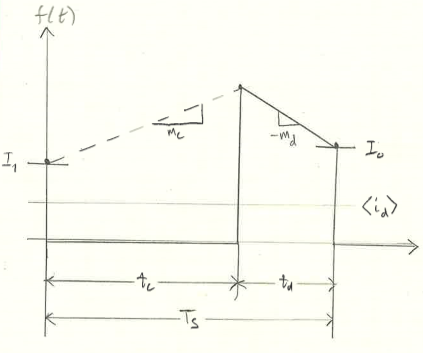
\includegraphics[width=0.95\linewidth]{Geometry.PNG}
    \caption{Geometry of the problem.}
    \label{Geometry}
\end{figure}

Above is a generalized plot of the charging and discharging current over one period where \(T_s\) is the period, \(I_1\) is the input current, \(I_0\) is the output current, \(m_c\) is the charging current slope, and \(-m_d\) is the discharging current slope. \(T_s\), \(I_1\), \(I_0\), \(m_c\), and \(-m_d\) are assumed to be known and the average currents, \(<i_c>\) and \(<i_d>\), for the period is what we are interested in solving for. The average currents over the period can be solved for by integrating the charging region for the charging current or the discharging region for the discharging current and averaging that over the entire period. Because of the simplicity of the structure of the problem, this integration can also be done geometrically by viewing the region as a triangle atop a rectangle. 
\subsection{Charging Current Solution}
\paragraph{}
For my solution I choose an integral approach to the problem. Based on the geometry of the problem I came up with the following integral: 
\begin{align}
    <i_c> = & \frac{1}{T_s}\int_0^{t_c}(m_ct+I_1)dt
\end{align}
This integral yields the following equation:
\begin{align}
    <i_c> = & I_1\frac{t_c}{T_s}+\frac{m_ct_c^2}{2T_s}
\end{align}
\paragraph{}
In the above equation every every variable is a known part of the problem exept for \(t_c\). This can be solved for geometrically by finding the intersection of the two lines. The location of this intersection on the x-axis will be \(t_c\). The charging and discharging slopes can be modeled as two lines using the equations:
\begin{align}
    f_c(t) & = m_ct+I_1\\
    f_d(t) & = -m_d(t-T_s)+I_0
\end{align}
Where \(f_c(t)\) is the value of the current from \(t = 0\) to \(t = t_c\) as a function of t and \(f_d(t)\) is the value of the current from \(t = 0\) to \(t = T_s\). Setting these two equations equal to each other will give a solution for t where the lines intersect. As can be seen in Figure \ref{Geometry}, the location of this intersection on the x-axis is \(t_c\).
\begin{align}
    f_c(t_c) & = f_d(t_c)\\
    m_ct+I_1 & = -m_d(t-T_s)+I_0\\
    t_c & = \frac{I_0-I_1+T_sm_d}{m_c+m_d}
\end{align}
\paragraph{}
Substituting equation (7) into equation (2) provides the following solution for \(<i_c>\):
\begin{align}
    <i_c> = & cI_0^2+dI_1^2+eI_0I_1+fI_0+gI_1+h\nonumber\\
    c = & \frac{m_c}{2T_sm_c^2+4T_sm_cm_d+2T_sm_d^2}\nonumber\\
    d = & \frac{m_c}{2T_sm_c^2+4T_sm_cm_d+2T_sm_d^2}-\frac{1}{T_sm_c+T_sm_d}\nonumber\\
    e = & \frac{1}{T_sm_c+T_sm_d}-\frac{m_c}{T_sm_c^2+2T_sm_cm_d+T_sm_d^2}\nonumber\\
    f = & \frac{m_cm_d}{m_c^2+2m_cm_d+m_d^2}\nonumber\\
    g = & \frac{m_d}{m_c+m_d}-\frac{m_cm_d}{m_c^2+2m_cm_d+m_d^2}\nonumber\\
    h = & \frac{T_sm_cm_d^2}{2m_c^2+4m_cm_d+2m_d^2}
\end{align}
\paragraph{}
This equation is powerful because \(T_s\), \(m_c\), and \(m_d\) are known constants and \(I_0\) and \(I_1\) are either known or inputs into the function depending on how the equation is being used.
\subsection{Discharging Current Solution}
\paragraph{}
The solution for the average discharging current is of the same form as the solution for the average charging current; only the coefficients are different. The integral equation for the discharging portion is as follows:
\begin{align}
    <i_d> = \frac{1}{T_s}\int_{t_c}^{T_s}(-m_d(t-T_s)+I_0)dt
\end{align}
This integral yields the following equation:
\begin{align}
    <i_d> = & I_0-I_0\frac{t_c}{Ts}+\frac{T_sm_d}{2}+\frac{m_dt_c^2}{2T_s}-m_dt_c\nonumber\\&+T_sm_d
\end{align}
\paragraph{}
Equation (10) is expressed in terms of \(t_c\) instead of \(t_d\) so that equation (7) can be reused in this calculation to find \(<i_d>\). This is possible using the equivalency: \(t_c = T_s-t_d\). The location of \(t_c\) can be found the same way as it was for the charging current, but because the problem has not changed, neither will \(t_c\). Substituting equation (7) into equation (10) provides the following solution for \(<i_d>\):
\begin{align}
    <i_d> = & cI_0^2+dI_1^2+eI_0I_1+fI_0+gI_1+h\nonumber\\
    c = & \frac{m_d}{2T_sm_c^2+4T_sm_cm_d+2T_sm_d^2}+\frac{1}{T_sm_c+T_sm_c}\nonumber\\
    d = & \frac{m_d}{2T_sm_c^2+4T_sm_cm_d+2T_sm_d^2}\nonumber\\
    e = & \frac{1}{T_sm_c+T_sm_d}-\frac{m_d}{T_sm_c^2+2T_sm_cm_d+T_sm_d^2}\nonumber\\
    f = & \frac{m_d^2}{m_c^2+2m_cm_d+m_d^2}-\frac{1-m_c}{m_c+m_d}\nonumber\\
    g = & \frac{1}{m_c+m_d}-\frac{m_d^2}{m_c^2+2m_cm_d+m_d^2}\nonumber\\
    h = & \frac{T_sm_d^3}{2m_c^2+4m_cm_d+2m_d^2}+\frac{T_sm_d^2}{m_c+m_d}+\frac{T_sm_d}{2}
\end{align}
\paragraph{}
Comparing equation (8) with equation (10), we can see that \(<i_c>\) and \(<i_d>\) are both quadratics of the same for with only the coefficients and constant being different between them.

%%%%%%%%%%%%%%%%%%%%%%%%%%%%%%%%%%%%%%%%%%%%%%%%%%%%%%%%%%%%%%%%%%%%%%%%%%%%%%%%%%%%%%%%%%%
% Model Validation Using Python and LTSpice
%%%%%%%%%%%%%%%%%%%%%%%%%%%%%%%%%%%%%%%%%%%%%%%%%%%%%%%%%%%%%%%%%%%%%%%%%%%%%%%%%%%%%%%%%%%
\section{Model Validation}
\paragraph{}
These equations were able to be verified using a LTSpice model and a Python script. The data was exported from LTSpice and plotted in Python over the output from the Python simulation to show their correlation.
\begin{figure}[!h]
    \centering
    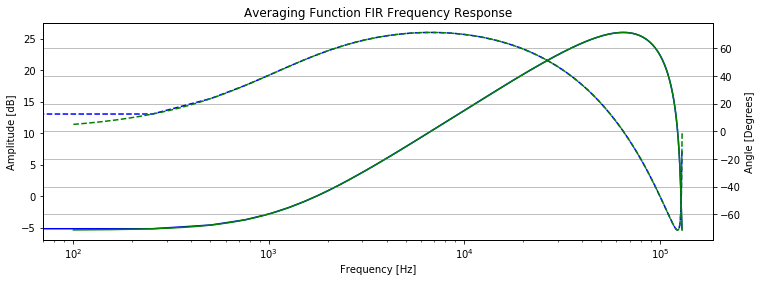
\includegraphics[width=0.95\linewidth]{PythonValidation.png}
    \caption{Python and LTSpice models.}
    \label{PythonValidation}
\end{figure}
% \subsection{LTSpice Results}
% \paragraph{}
% \paragrpah{}
% \begin{figure}[!h]
%     \centering
%     \includegraphics[width=0.95\linewidth]{LTSpiceOutput.pdf}
%     \caption{Output from LTSpice.}
%     \label{LTSpiceOutput}
% \end{figure}
% \paragraph{}
% \begin{figure}[!h]
%     \centering
%     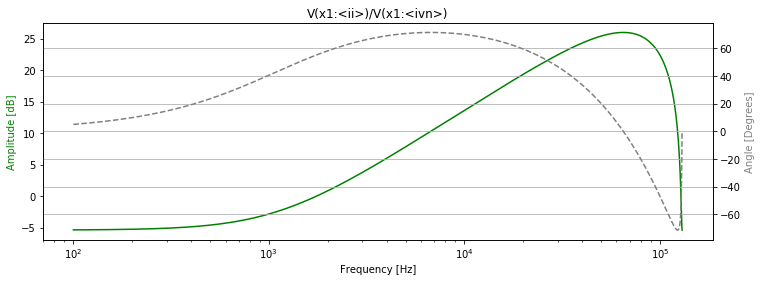
\includegraphics[width=0.95\linewidth]{LTSpiceOutputPython.png}
%     \caption{Output from LTSpice plotted in Python.}
%     \label{LTSpiceOutputPython}
% \end{figure}
% \subsection{Python Results}
% \paragraph{}
% \begin{figure}[!h]
%     \centering
%     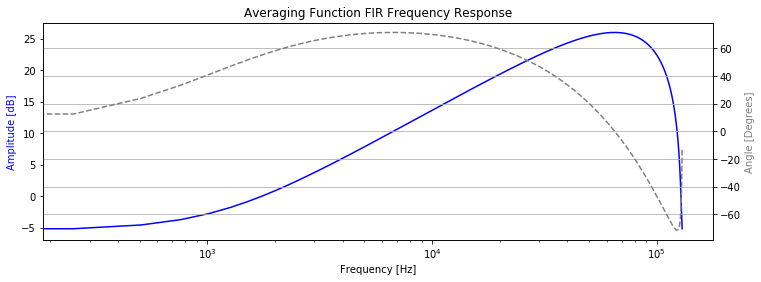
\includegraphics[width=0.95\linewidth]{PythonOutput.png}
%     \caption{Output from Python}
%     \label{PythonOutput}
% \end{figure}
% \subsection{Results Compared}
% \paragraph{}
% To compare the output from LTSpice with the output from Python, the raw data had to first be exported from LTSpice. It was ran through a Python script to convert the data from one long string, to several arrays that can be plotted. This was then combined with the output from the Python script for the average charging current and both data sets were plotted on top of each other.
% \paragraph{}
% \begin{figure}[!h]
%     \centering
%     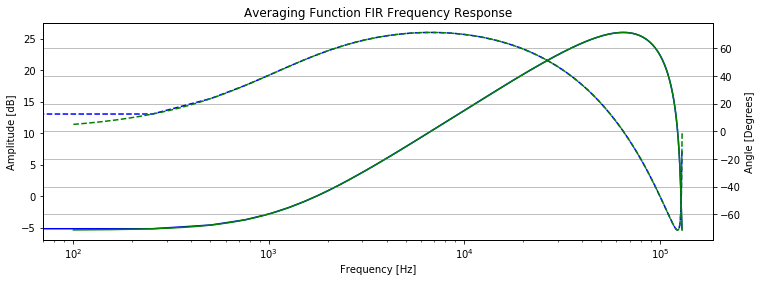
\includegraphics[width=0.95\linewidth]{PythonValidation.png}
%     \caption{Python and LTSpice models.}
%     \label{PythonValidation}
% \end{figure}
% \paragraph{}
% Above you can see the LTSpice data in green plotted on top of the Python data in blue.

%%%%%%%%%%%%%%%%%%%%%%%%%%%%%%%%%%%%%%%%%%%%%%%%%%%%%%%%%%%%%%%%%%%%%%%%%%%%%%%%%%%%%%%%%%%
% Small Signal Model
%%%%%%%%%%%%%%%%%%%%%%%%%%%%%%%%%%%%%%%%%%%%%%%%%%%%%%%%%%%%%%%%%%%%%%%%%%%%%%%%%%%%%%%%%%%
\section{Small Signal Model}
\paragraph{}
In the small signal model, \(i_0=I_0+\Delta_0\) and \(i_1=I_1+\Delta_1\), where \(i_0\) and \(i_1\) refer to the small signal currents for time [t] and [t-1] and \(\Delta_0\) and \(\Delta_1\) refer to the small variation \(i\) has from \(I\). To analyze the small signal analysis we can use this relationship and the following equations:
% \begin{align}
%     <i_x> = & ci_0^2+di_1^2+ei_0i_1+fi_0+gi_1+h
% \end{align}
% \paragraph{}
% I substituted \(I_0+\Delta_0\) for \(i_0\) and \(I_1+\Delta_1\) for \(i_1\) and used the following equalities:
% \begin{align}
%     \Delta_0^2 \approx & 2\Delta_0 |_{\Delta_0<<1}\\
%     \Delta_0\Delta_1 \approx & \Delta_0+\Delta_1 |_{\Delta_0<<1, \Delta_1<<1}
% \end{align}
% This resulted in the following equation:
% \begin{align}
%     <i_c & = \Delta
% \end{align}

% Add section explaining I0 and I1 are valley currents.
% Ratio of area changing with respect to a small change (Delta) in I (valley current).

\onecolumn

%\newpage
%\bibliographystyle{apacite}
%\bibliography{references}

\end{document}